\section{Linear Programming and Integer Linear Programming}

\subsection{Linear Programming}

Linear programming is about satisfying a list of constraints rappresented by some equations, the general formula being:

\[min/max \; c^{t}x\]
\[\begin{cases} Ax \geq b \\ x \geq 0 \; or \; x \leq 0 \end{cases}\]

where $c^{t}x$ is the objective function that could either be maximized or minimized, A is a matrix $m \; x \; n$ and the variables $x_{i}$ could either be positive or negative, there exists many algorithms to solve LP problems in poly-time, the most famous is the simplex algorithm or the graphic method(please note that, in order to use the graphic method, you must have 2 variables maximum in the problem).

\subsection{Primal-Dual}
supposing we have a primal problem in the form of:

\[min \; c^{t}x\]
\[\begin{cases} Ax \geq b \\ x \geq 0 \end{cases}\]

the the dual problem will be:

\[max \; b^{t}y\]
\[\begin{cases} A^{t}y \leq c \\ y \geq 0 \end{cases}\]

The objective function change from maximize to minimize and vice-versa, while the matrix inequalities changes to the opposite from the primal to the dual, a practical example:

\[min \; 7x1 + x2 + 5x3\]
\[\begin{cases} x1-x2+3x3 \geq 10 \\ 5x1+2x2-x3 \geq 6 \\ x1,x2,x3 \geq 0 \end{cases}\]

becomes:

\[max \; 10y1 + 6y2\]
\[\begin{cases} y1+5y2 \leq 7 \\ -y1 + 2y2 \leq 1 \\ 3y1-y2 \leq 5 \\y1,y2 \geq 0 \end{cases}\]

Why are there so important?\\

\emph{Primal-Dual Weak Theorem}: If x is feasible for the Primal and y is feasible for the Dual, then:

\[ \sum^{n}_{j=1} c_{j}x_{j} \geq \sum^{m}_{i=1}b_{i}y_{i}\]

basically the solution of the primal is always greater than the solution of the dual.\\\\
\emph{Primal-Dual Strong Theorem}: If the Primal has finite optimum then the Dual has finite optimum. Let $x^{∗}$ and $y^{∗}$ be the primal and the dual optimum solutions. Then:

\[ \sum^{n}_{j=1} c_{j}x_{j}^{*} = \sum^{m}_{i=1}b_{i}y_{i}^{*}\]

\subsection{Integer Linear Programming}

Same as linear programming, but this time x variables can only be either 1 or 0:

\[min \; c^{t}x\]
\[\begin{cases} Ax \geq 1 \\ x = \{0,1\} \end{cases}\]

Unfortunately it does not exists a poly-time algorithm to solve ILP problems.\\

\emph{Transformation from ILP to LP}: in order to transform an ILP problem to LP we need to use a process called relaxation, so we need to transform the original ILP problem into:

\[min \; c^{t}x\]
\[\begin{cases} Ax \geq 1 \\ x = [0,1] \end{cases}\]

\emph{Transformation from LP to ILP}: in order to transform an LP problem to ILP we need to use a process called rounding: given the solution of LP problem, we need to round some values to 1 or to 0, a simple method will be $x_{ILP} = 1 \; if \; x_{LP} \geq 1/2$ and $x_{ILP} = 0 \; if \; x_{LP} \leq 1/2$ but there also exists some more sophisticated methods involving probabilities.\\

\emph{Integrality Gap}: largest ratio on all instances between the optimum integral solution and the optimum relaxed solution.

\subsection{Weighted Vertex Cover with ILP}

Given a graph G = (V, E) with vertex weights $w_{i} \geq 0$, find a min-weight subset of vertices $S \subseteq V$ such that every edge is incident to at least one vertex in S.

\begin{figure}[H]
    \centering
    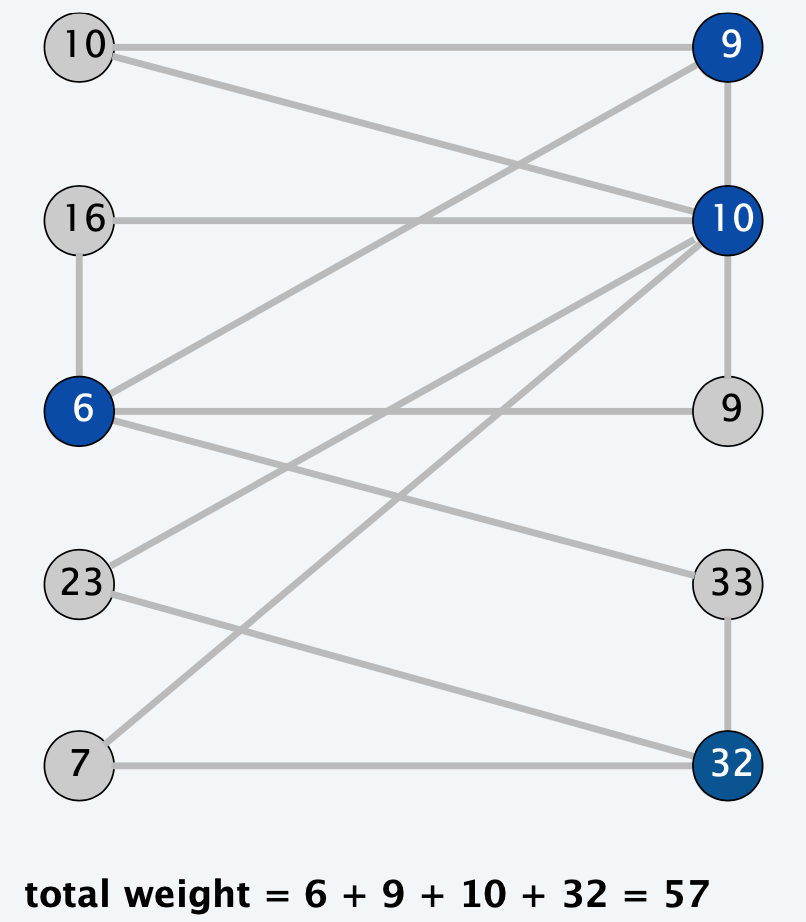
\includegraphics[width=0.3\textwidth ]{wVertexCover}
    \caption{Instance of weighted vertex cover}
\end{figure}

So in order to formulate the problem, we assign to the variable $x_{i}$ 1 if is in the vertex cover, 0 if not, while the objective function is to minimize $\sum_{i} w_{i}x_{i}$.


\[min \; \sum_{i} w_{i}x_{i}\]
\[\begin{cases} x_{i} + x_{j} \geq 1 \; \forall (i,j) \in E \\ x = \{0,1\} \; \forall i \in V\end{cases}\]

obviously $x_{i}+x_{j} \geq 1$ because if I take the vertex i, i must also take the vertex j, in order to solve the problem we need to relax it:

\[min \; \sum_{i} w_{i}x_{i}\]
\[\begin{cases} x_{i} + x_{j} \geq 1 \; \forall (i,j) \in E \\ x \geq 0 \; \forall i \in V\end{cases}\]

So, as said before, we need to round the fractional values in the LP solution, if $x \geq 1/2 \Rightarrow x^{*} = 1$ else $x \leq 1/2 \Rightarrow x^{*} = 0$

\begin{claim}
    The rounded LP solution is a 2approximation for the optimum ILP solution.
\end{claim}

\begin{proof}
    Let $S^{*}$ be optimal vertex cover. Then:
    \[\sum_{i \in S^{*}} w_{i} \geq \sum_{i \in S}w_{i}x_{i}^{*} \geq 1/2 \sum_{i \in S}w_{i}\]
\end{proof}

\subsection{Generalized Load Balancing}
Same as 9.1 but this time, not all machines are authorized: job $j \in J$ must run contiguously on an authorized machine in $M_{j} \subseteq M$, being $x_{ij}$ the times the machine i spends processing the job j:

\begin{figure}[H]
    \centering
    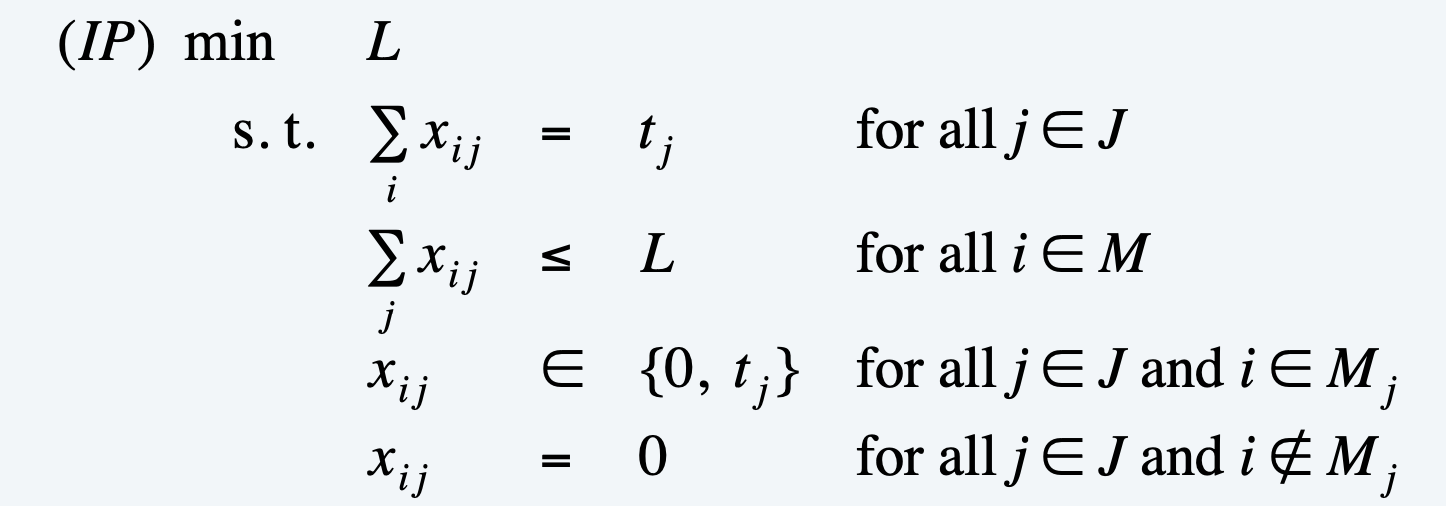
\includegraphics[width=0.6\textwidth ]{gILP}
\end{figure}

\begin{figure}[H]
    \centering
    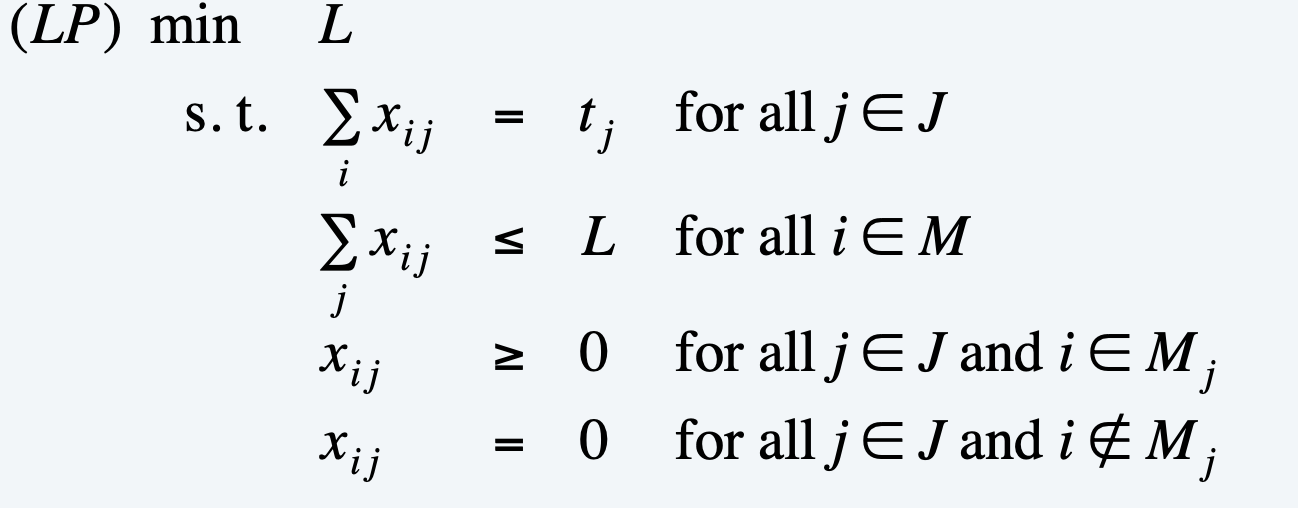
\includegraphics[width=0.6\textwidth ]{gLP}
\end{figure}

\begin{claim}
    The optimal makespan $L^{*} ≥ max_{j} t_{j}$
\end{claim}
\begin{proof}
    Some machine must process the most time-consuming job
\end{proof}\\
\begin{claim}
    Let L be optimal value to the LP. Then, optimal makespan $L^{*} \geq L$.
\end{claim}\\
\begin{proof}
    LP has fewer constraints than ILP formulation.
\end{proof}
